\section{Flow Matching}

上一章中，我们已经把 flow model 写成由神经网络参数化的 ODE：
\begin{equation}
X_0 \sim p_{\mathrm{init}}, \qquad
\frac{\dd X_t}{\dd t}=u_t^\theta(X_t).
\end{equation}
采样时，只要从简单分布 $p_{\mathrm{init}}$ 取一个初始点，再沿着这个 ODE 模拟到 $t=1$，就得到输出 $X_1$。
因此，训练问题可以表述为：如何学习向量场 $u_t^\theta$，使得 $X_1 \sim \data$。

\subsection{条件概率路径与边缘概率路径}

我们希望模型把初始分布 $p_{\mathrm{init}}$ 连续地变成数据分布 $\data$。
为了描述这个连续变化过程，引入\emph{概率路径}。

\begin{definition}[条件概率路径]
给定数据点 $z \in \R^d$，一族条件分布 $p_t(\cdot|z)$ 称为从 $p_{\mathrm{init}}$ 到 $\delta_{z}$ 的条件概率路径，如果对所有 $z$ 都有
\begin{equation}
p_0(\cdot|z)=p_{\mathrm{init}},
\qquad
p_1(\cdot|z)=\delta_{z}.
\end{equation}
其中 $\delta_{z}$ 表示集中在 $z$ 处的 Dirac 分布。
\end{definition}

直观上，$p_t(\cdot|z)$ 描述的是：如果最终目标是某个固定数据点 $z$，那么在中间时刻 $t$，样本应该分布在哪里。
当 $t=0$ 时，它还是纯噪声；当 $t=1$ 时，它退化为确定的数据点 $z$。

由条件概率路径可以推导出边缘概率路径。
采样方式是先从数据分布中采样一个数据点，再从对应的条件路径中采样：
\begin{equation}
z \sim \data,
\qquad
x \sim p_t(\cdot|z)
\quad \Longrightarrow \quad
x \sim p_t.
\end{equation}
如果写成密度形式，则有
\begin{equation}
p_t(x)=\int p_t(x|z)\data(z)\,\dd z.
\end{equation}

由于条件路径端点满足 $ p_0(\cdot|z)=p_{\mathrm{init}}, \quad p_1(\cdot|z)=\delta_{z}$，在 $t=0$ 时有：
\begin{equation}
  p_0(x)=\int p_{\mathrm{init}}(x)\data(z)\,dz = p_{\mathrm{init}}
\end{equation}
在 $t=1$ 时有：
\begin{equation}
  p_1(x)=\int \delta(x-z)\data(z)\,dz = \data
\end{equation}


\begin{equation}
p_0=p_{\mathrm{init}},
\qquad
p_1=\data.
\end{equation}
也就是说，$p_t$ 正是我们想让模型轨迹边缘分布遵循的噪声到数据的插值过程。

\begin{example}[Gaussian 条件概率路径]
最常用的一类条件概率路径是 Gaussian path。令 $\alpha_t,\beta_t$ 为两个连续可微的调度函数，满足
\begin{equation}
\alpha_0=0,\quad \alpha_1=1,
\qquad
\beta_0=1,\quad \beta_1=0.
\end{equation}
定义
\begin{equation}
p_t(\cdot|z)=\Normal(\alpha_t z,\beta_t^2 I_d).
\end{equation}
于是 $t=0$ 时有
\begin{equation}
p_0(\cdot|z)=\Normal(0,I_d)=p_{\mathrm{init}},
\end{equation}
而 $t=1$ 时有
\begin{equation}
p_1(\cdot|z)=\Normal(z,0)=\delta_{z}.
\end{equation}
因此这是一个合法的条件概率路径。
实际采样时可以写成
\begin{equation}
\varepsilon \sim \Normal(0,I_d),
\qquad
x_t=\alpha_t z+\beta_t \varepsilon.
\end{equation}
当 $t$ 较小时，$x_t$ 主要由噪声组成；当 $t$ 接近 $1$ 时，$x_t$ 逐渐接近数据点 $z$。
\end{example}

\begin{figure}[htbp]
  \centering
  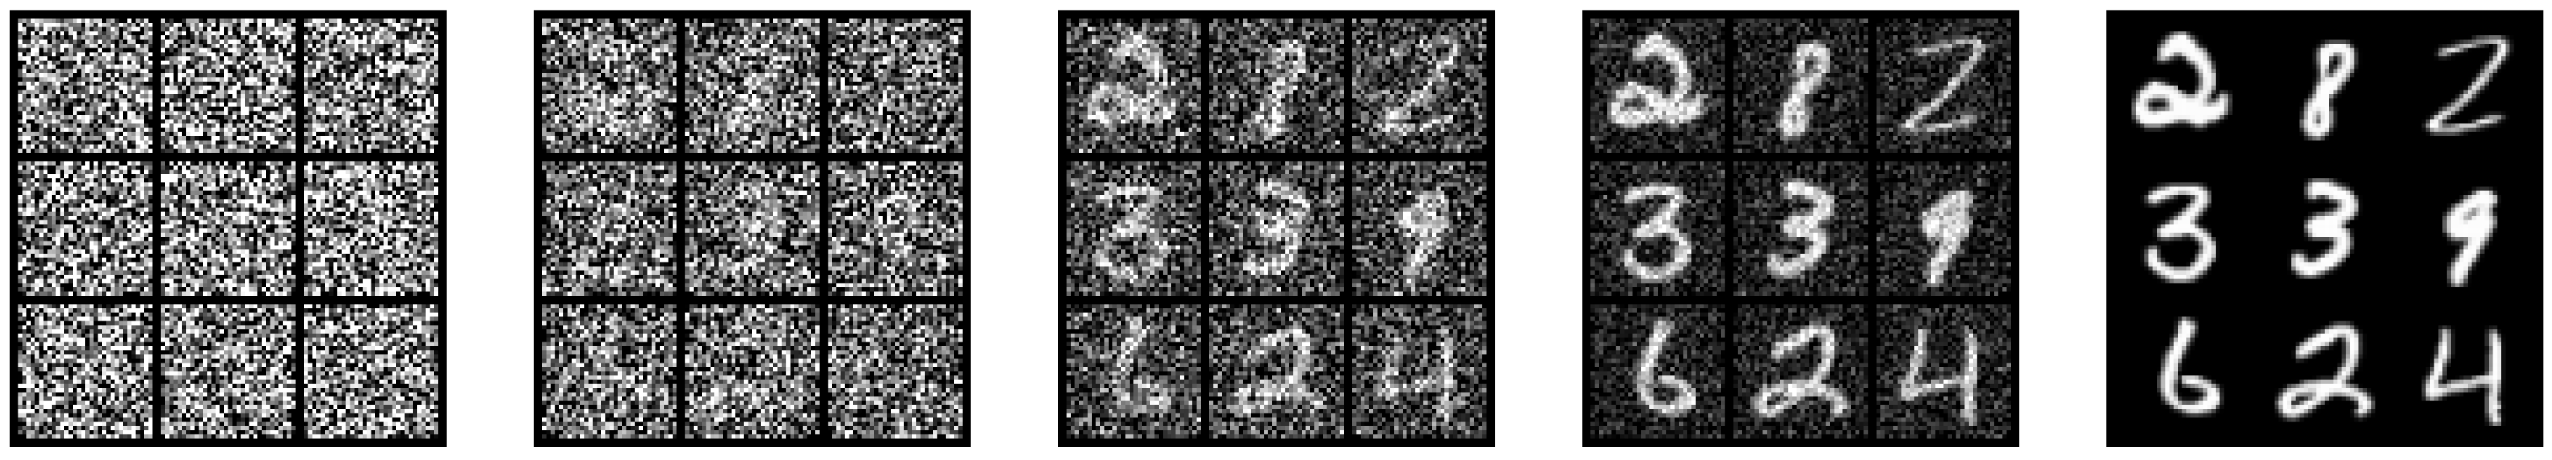
\includegraphics[width=0.82\linewidth]{tex/figures/selected/figure04-gaussian-path-images.png}
  \caption{Gaussian 条件概率路径在图像数据上的直观效果：从纯噪声逐渐插值到数据样本。}
  \label{fig:gaussian-path-images}
\end{figure}

图~\ref{fig:gaussian-path-images} 展示了 Gaussian path 的核心直觉：较小的 $t$ 对应更多噪声，较大的 $t$ 对应更接近真实数据的样本。

\begin{figure}[htbp]
  \centering
  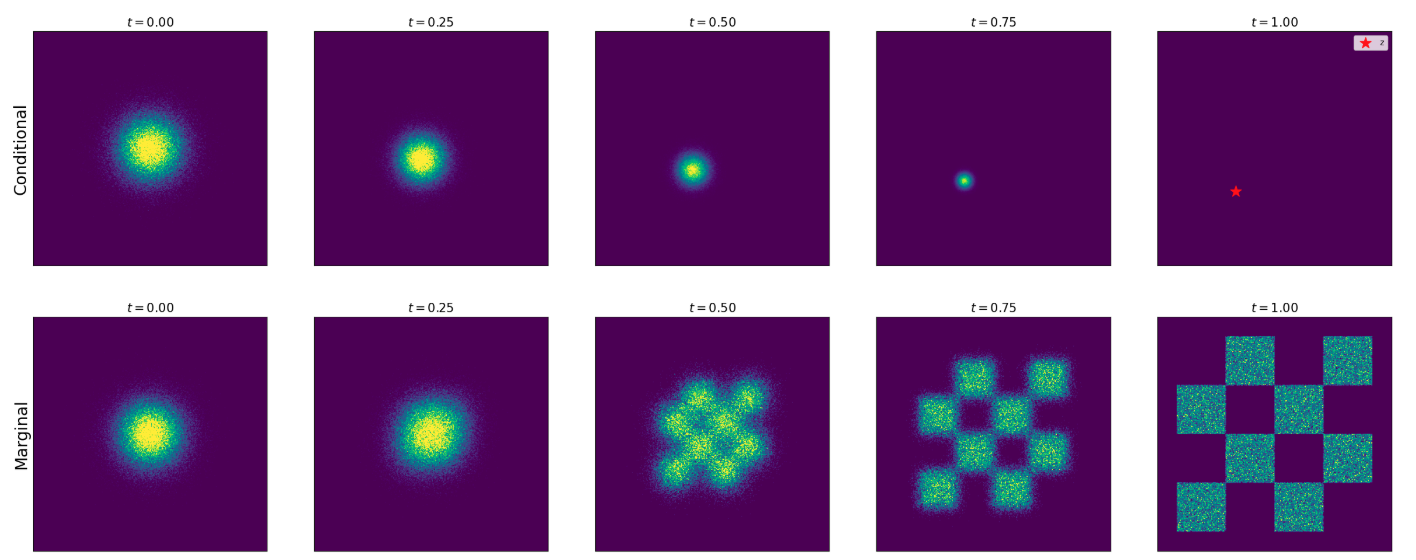
\includegraphics[width=0.95\linewidth]{tex/figures/selected/figure05-paths.png}
  \caption{条件概率路径与边缘概率路径。上排固定数据点 $z$，下排对数据分布 $\data$ 做边缘化。}
  \label{fig:conditional-marginal-paths}
\end{figure}

图~\ref{fig:conditional-marginal-paths} 对比了条件路径和边缘路径：条件路径以单个数据点为终点，而边缘路径以整个数据分布为终点。

\subsection{条件向量场与边缘向量场}

概率路径只说明了每个时刻的目标分布是什么，还没有说明应该用什么 ODE 到达这些分布。
Flow Matching 接下来要构造一个目标向量场，使得 ODE 轨迹的边缘分布正好沿着 $p_t$ 演化。

\begin{definition}[条件向量场]
对固定数据点 $z$，若向量场 $u_t^{\mathrm{target}}(x|z)$ 对应的 ODE 满足
\begin{equation}
X_0 \sim p_{\mathrm{init}},
\qquad
\frac{\dd X_t}{\dd t}
=u_t^{\mathrm{target}}(X_t|z)
\quad \Longrightarrow \quad
X_t \sim p_t(\cdot|z),
\end{equation}
则称 $u_t^{\mathrm{target}}(\cdot|z)$ 是条件概率路径 $p_t(\cdot|z)$ 的条件向量场。
\end{definition}

条件向量场本身并不能直接生成新样本，因为它依赖某个已经给定的数据点 $z$。
但它可以作为构造真实生成向量场的基本部件。

\begin{theorem}[边缘化技巧]
设 $u_t^{\mathrm{target}}(x|z)$ 是条件概率路径 $p_t(\cdot|z)$ 的条件向量场。
定义边缘向量场
\begin{equation}
u_t^{\mathrm{target}}(x)
=
\int
u_t^{\mathrm{target}}(x|z)
\frac{p_t(x|z)\data(z)}{p_t(x)}
\,\dd z.
\end{equation}
则由该向量场定义的 ODE 满足
\begin{equation}
X_0 \sim p_{\mathrm{init}},
\qquad
\frac{\dd X_t}{\dd t}
=u_t^{\mathrm{target}}(X_t)
\quad \Longrightarrow \quad
X_t \sim p_t.
\end{equation}
特别地，$X_1 \sim \data$。
\label{thm:marginal_skill}
\end{theorem}

这个公式可以理解为一个后验加权平均。
给定当前点 $x$，项
\begin{equation}
\frac{p_t(x|z)\data(z)}{p_t(x)}
\end{equation}
描述了“当前 $x$ 可能来自哪个数据点 $z$”的后验权重，即 $p_t(z|x)$。
边缘向量场就是把所有条件向量场 $u_t^{\mathrm{target}}(x|z)$ 按照这个权重平均起来。

\begin{figure}[htbp]
  \centering
  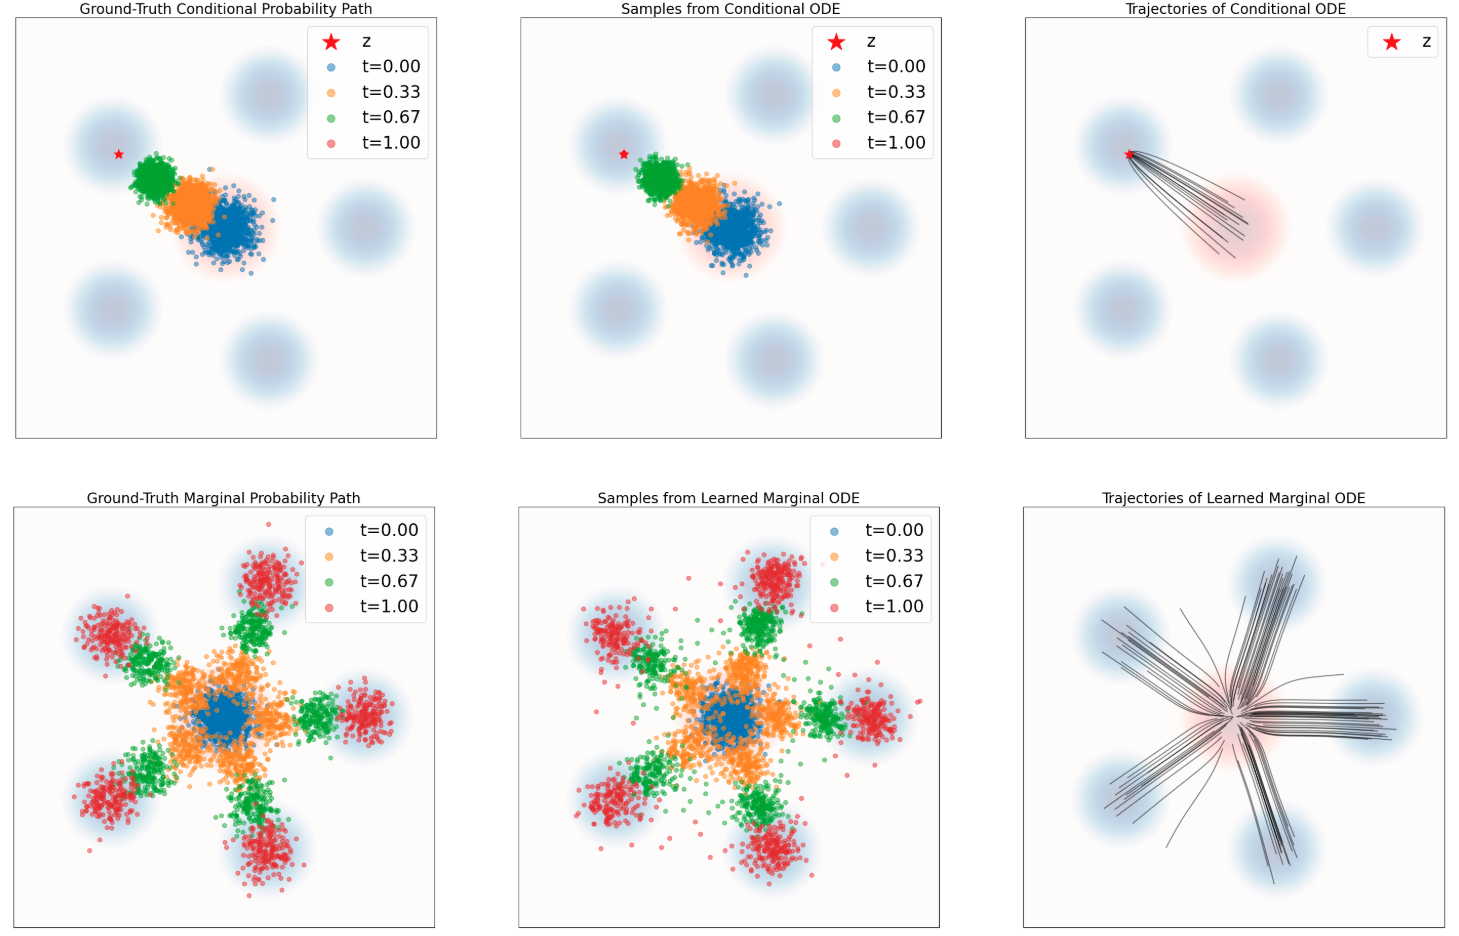
\includegraphics[width=0.95\linewidth]{tex/figures/selected/figure06-ode-paths.png}
  \caption{用 ODE 模拟条件概率路径和边缘概率路径。上排对应固定数据点的条件路径，下排对应边缘路径。}
  \label{fig:ode-path-simulation}
\end{figure}

图~\ref{fig:ode-path-simulation} 展示了边缘化技巧的作用：虽然条件向量场只会把样本推向固定数据点，但对条件向量场做后验加权平均后，可以得到真正生成数据分布的边缘向量场。

为了说明为什么这个构造是正确的，我们引入连续性方程。
\begin{theorem}[连续性方程]
设 $u_t(x)$ 是一个足够光滑的时间依赖向量场，$X_0 \sim p_{\mathrm{init}}$，且随机变量 $X_t$ 满足
\begin{equation}
\frac{\dd X_t}{\dd t}=u_t(X_t).
\end{equation}
则 $X_t \sim p_t(x)$ 当且仅当 $p_t$ 满足
\begin{equation}
\begin{aligned}
\partial_t p_t(x)
&=
-\divergence\!\left(p_tu_t^{\mathrm{target}}\right)\left(x\right)
& \qquad\qquad\qquad\qquad \blacktriangleright \: \makebox[3cm][l]{\text{连续性方程}} \\
&=
-\sum_{i=1}^d \frac{\partial}{\partial{x_i}}\!\left(p_tu_t^{\mathrm{target}}\right)\left(x\right)
& \qquad\qquad\qquad\qquad \blacktriangleright \: \makebox[3cm][l]{\text{分量形式}}
\end{aligned}
\end{equation}

\end{theorem}

连续性方程描述的是概率质量如何在向量场的推动下在空间中流动。左边 $\partial_t p_t(x)$ 表示位置 $x$ 处概率密度随时间的变化率，右边则表示概率流 $p_t(x)u_t(x)$ 的净流出。这里
\begin{equation}
\divergence\!\left(v_t\right)\left(x\right)=\sum_{i=1}^d \frac{\partial}{\partial{x_i}}v_t^i(x)
\end{equation}
是 $v_t$ 的散度定义。下面我们用连续性方程证明~\ref{thm:marginal_skill}。

\begin{proof}
对每个固定的 $z$，条件向量场 $u_t^{\mathrm{target}}(x|z)$ 使得条件密度 $p_t(\cdot|z)$ 满足连续性方程，因此
\begin{equation}
\begin{aligned}
\partial_t p_t(x)
&=
\int \partial_t p_t(x|z)\data(z)\,\dd z
& \qquad\qquad \blacktriangleright \: \makebox[3.2cm][l]{\text{边缘密度定义}} \\
&=
-\int
\divergence\!\left(
p_t(x|z)\,u_t^{\mathrm{target}}(x|z)
\right)\data(z)\,\dd z
& \qquad\qquad \blacktriangleright \: \makebox[3.2cm][l]{\text{条件连续性方程}} \\
&=
-\divergence\!\left(
\int
p_t(x|z)\,u_t^{\mathrm{target}}(x|z)\data(z)\,\dd z
\right)
& \qquad\qquad \blacktriangleright \: \makebox[3.2cm][l]{\text{散度只对 $x$ 作用}} \\
&=
-\divergence\!\left(
p_t(x)
\int
u_t^{\mathrm{target}}(x|z)
\frac{p_t(x|z)\data(z)}{p_t(x)}
\,\dd z
\right)
& \qquad\qquad \blacktriangleright \: \makebox[3.2cm][l]{\text{数学变换}} \\
&=
-\divergence\!\left(
p_t(x)\,u_t^{\mathrm{target}}(x)
\right)
& \qquad\qquad \blacktriangleright \: \makebox[3.2cm][l]{\text{边缘向量场定义}}
\end{aligned}
\end{equation}
因此 $p_t$ 满足向量场 $u_t^{\mathrm{target}}(x)$ 所对应的连续性方程。再结合初值 $p_0=p_{\mathrm{init}}$，可知由
\begin{equation}
X_0 \sim p_{\mathrm{init}},
\qquad
\frac{\dd X_t}{\dd t}=u_t^{\mathrm{target}}(X_t)
\end{equation}
定义的轨迹在任意时刻都满足 $X_t \sim p_t$，特别地
\begin{equation}
X_1 \sim p_1=\data.
\end{equation}
\end{proof}





\begin{example}[Gaussian probability path 的目标 ODE]
考虑
\begin{equation}
p_t(\cdot|z)=\Normal(\alpha_t z,\beta_t^2 I_d).
\end{equation}
其中 $\alpha_t,\beta_t$ 是给定的噪声调度函数，满足
\begin{equation}
\alpha_0=\beta_1=0,\qquad \alpha_1=\beta_0=1.
\end{equation}
记 $\dot{\alpha}_t=\frac{\dd}{\dd t}\alpha_t$，$\dot{\beta}_t=\frac{\dd}{\dd t}\beta_t$。

我们先定义条件 flow
\begin{equation}
\psi_t^{\mathrm{target}}(x|z)=\alpha_t z+\beta_t x.
\end{equation}
若 $X_0\sim p_{\mathrm{init}}=\Normal(0,I_d)$，则
\begin{equation}
X_t=\psi_t^{\mathrm{target}}(X_0|z)=\alpha_t z+\beta_t X_0
\sim
\Normal(\alpha_t z,\beta_t^2 I_d),
\end{equation}
\noindent
因此该 flow 诱导出了条件概率路径 $p_t(\cdot|z)$。再由
\begin{equation}
\begin{aligned}
\frac{\dd}{\dd t}\psi_t^{\mathrm{target}}(x|z)
&=
u_t^{\mathrm{target}}
\bigl(
\psi_t^{\mathrm{target}}(x|z)| z
\bigr)
\qquad
\text{for all } x,z \in \mathbb{R}^d \\
\dot{\alpha}_t z + \dot{\beta}_t x
&=
u_t^{\mathrm{target}}
\bigl(
\alpha_t z + \beta_t x | z
\bigr)
\qquad
\text{for all } x,z \in \mathbb{R}^d \\
\dot{\alpha}_t z
+
\dot{\beta}_t
\left(
\frac{x - \alpha_t z}{\beta_t}
\right)
&=
u_t^{\mathrm{target}}(x | z)
\qquad
\text{for all } x,z \in \mathbb{R}^d \\
\left(
\dot{\alpha}_t
-
\frac{\dot{\beta}_t}{\beta_t}\alpha_t
\right) z
+
\frac{\dot{\beta}_t}{\beta_t}x
&=
u_t^{\mathrm{target}}(x | z)
\qquad
\text{for all } x,z \in \mathbb{R}^d
\end{aligned}
\end{equation}

因此，若考虑 ODE
\begin{equation}
X_0\sim \Normal(0,I_d),
\qquad
\frac{\dd X_t}{\dd t}=u_t^{\mathrm{target}}(X_t|z),
\end{equation}
则它的解满足
\begin{equation}
X_t\sim \Normal(\alpha_t z,\beta_t^2 I_d).
\end{equation}
\end{example}

\subsection{学习边缘向量场}

现在的问题变成：如何用神经网络 $u_t^\theta$ 学习边缘向量场 $u_t^{\mathrm{target}}$？
最直接的想法是最小化均方误差
\begin{equation}
\mathcal{L}_{\mathrm{FM}}(\theta)
=
\E_{t\sim \mathrm{Unif}[0,1],\,x\sim p_t}
\left[
\left\|
u_t^\theta(x)-u_t^{\mathrm{target}}(x)
\right\|^2
\right].
\end{equation}
这个损失称为 Flow Matching loss。
如果能够最小化它，神经网络就会逼近真正的边缘向量场，从而在采样时把 $p_{\mathrm{init}}$ 推到 $\data$。

但实际中 $u_t^{\mathrm{target}}(x)$ 很难直接计算，因为它包含对整个数据分布的积分。
相比之下，条件向量场 $u_t^{\mathrm{target}}(x|z)$ 往往有解析形式。
因此定义 Conditional Flow Matching loss：
\begin{equation}
\mathcal{L}_{\mathrm{CFM}}(\theta)
=
\E_{t\sim \mathrm{Unif}[0,1],\,z\sim \data,\,x\sim p_t(\cdot|z)}
\left[
\left\|
u_t^\theta(x)-u_t^{\mathrm{target}}(x|z)
\right\|^2
\right].
\end{equation}

\begin{theorem}[Conditional Flow Matching]
\label{thm:flow_matching_loss}
Flow Matching loss 与 Conditional Flow Matching loss 只相差一个与参数 $\theta$ 无关的常数：
\begin{equation*}
\mathcal{L}_{\mathrm{FM}}(\theta)
=
\mathcal{L}_{\mathrm{CFM}}(\theta)+C.
\end{equation*}
因此二者关于 $\theta$ 的梯度相同：
\begin{equation*}
\nabla_\theta \mathcal{L}_{\mathrm{FM}}(\theta)
=
\nabla_\theta \mathcal{L}_{\mathrm{CFM}}(\theta).
\end{equation*}
也就是说，最小化可计算的 $\mathcal{L}_{\mathrm{CFM}}$，等价于最小化理想但不可直接计算的 $\mathcal{L}_{\mathrm{FM}}$。
\end{theorem}

\begin{proof}
从 Flow Matching loss 出发，
\begin{equation*}
\begin{aligned}
\mathcal{L}_{\mathrm{FM}}(\theta)
&\overset{(i)}{=}
\mathbb{E}_{t \sim \mathrm{Unif},\, x \sim p_t}
\left[
\left\|
u_t^\theta(x)
-
u_t^{\mathrm{target}}(x)
\right\|^2
\right] \\
&\overset{(ii)}{=}
\mathbb{E}_{t \sim \mathrm{Unif},\, x \sim p_t}
\left[
\left\|
u_t^\theta(x)
\right\|^2
-
2\,u_t^\theta(x)^{T}
u_t^{\mathrm{target}}(x)
+
\left\|
u_t^{\mathrm{target}}(x)
\right\|^2
\right] \\
&\overset{(iii)}{=}
\mathbb{E}_{t \sim \mathrm{Unif},\, x \sim p_t}
\left[
\left\|
u_t^\theta(x)
\right\|^2
\right]
-
2\,
\mathbb{E}_{t \sim \mathrm{Unif},\, x \sim p_t}
\left[
u_t^\theta(x)^{T}
u_t^{\mathrm{target}}(x)
\right]
+
\underbrace{
\mathbb{E}_{t \sim \mathrm{Unif}_{[0,1]},\, x \sim p_t}
\left[
\left\|
u_t^{\mathrm{target}}(x)
\right\|^2
\right]
}_{=:C_1} \\
&\overset{(iv)}{=}
\mathbb{E}_{t \sim \mathrm{Unif},\, z \sim \data,\, x \sim p_t(\cdot \mid z)}
\left[
\left\|
u_t^\theta(x)
\right\|^2
\right]
-
2\,
\mathbb{E}_{t \sim \mathrm{Unif},\, x \sim p_t}
\left[
u_t^\theta(x)^{T}
u_t^{\mathrm{target}}(x)
\right]
+
C_1
\end{aligned}
\end{equation*}
其中在 $(iii)$ 由于第三项和模型参数 $\theta$ 无关，我们用常数 $C_1$ 来表示；在 $(iv)$ 由于 $p_t$ 是由条件概率路径边缘化得到的，我们可以把期望中的 $x \sim p_t$ 替换成先采样 $z \sim \data$ 再采样 $x \sim p_t(\cdot|z)$。对于第二项
\begin{equation*}
\begin{aligned}
\mathbb{E}_{t \sim \mathrm{Unif},\, x \sim p_t}
\left[
u_t^\theta(x)^T
u_t^{\mathrm{target}}(x)
\right]
&\overset{(i)}{=}
\int_0^1
\int
p_t(x)\,
u_t^\theta(x)^T
u_t^{\mathrm{target}}(x)
\,dx\,dt \\
&\overset{(ii)}{=}
\int_0^1
\int
p_t(x)\,
u_t^\theta(x)^T
\left[
\int
u_t^{\mathrm{target}}(x \mid z)
\frac{
p_t(x \mid z)\,
\data(z)
}{
p_t(x)
}
\,dz
\right]
dx\,dt \\
&\overset{(iii)}{=}
\int_0^1
\int
\int
u_t^\theta(x)^T
u_t^{\mathrm{target}}(x \mid z)\,
p_t(x \mid z)\,
\data(z)
\,dz\,dx\,dt \\
&\overset{(iv)}{=}
\mathbb{E}_{t \sim \mathrm{Unif},\, z \sim \data,\, x \sim p_t(\cdot \mid z)}
\left[
u_t^\theta(x)^T
u_t^{\mathrm{target}}(x \mid z)
\right]
\end{aligned}
\end{equation*}
其中 $(iv)$ 将积分形式表达成期望形式。
因此
\begin{equation*}
\begin{aligned}
\mathcal{L}_{\mathrm{FM}}(\theta) & \overset{(i)}{=} \mathbb{E}_{t \sim \text{Unif}, z \sim \data, x \sim p_t(\cdot | z)}\left[\|u_t^\theta(x)\|^2\right] - 2\mathbb{E}_{t \sim \text{Unif}, z \sim \data, x \sim p_t(\cdot | z)}\left[u_t^\theta(x)^T u_t^{\mathrm{target}}(x | z)\right] + C_1 \\
& \overset{(ii)}{=} \mathbb{E}_{t \sim \text{Unif}, z \sim \data, x \sim p_t(\cdot | z)}\left[\|u_t^\theta(x)\|^2 - 2u_t^\theta(x)^T u_t^{\mathrm{target}}(x | z) + \|u_t^{\mathrm{target}}(x | z)\|^2 - \|u_t^{\mathrm{target}}(x | z)\|^2\right] + C_1 \\
& \overset{(iii)}{=} \mathbb{E}_{t \sim \text{Unif}, z \sim \data, x \sim p_t(\cdot | z)}\left[\|u_t^\theta(x) - u_t^{\mathrm{target}}(x | z)\|^2\right] + \underbrace{\mathbb{E}_{t \sim \text{Unif}, z \sim \data, x \sim p_t(\cdot | z)}\left[-\|u_t^{\mathrm{target}}(x | z)\|^2\right]}_{C_2} + C_1 \\
& \overset{(iv)}{=} \mathcal{L}_{\mathrm{CFM}}(\theta) + \underbrace{C_2 + C_1}_{=: C}
\end{aligned}
\end{equation*}
因此
\[
\nabla_\theta \mathcal{L}_{\mathrm{FM}}(\theta)
=
\nabla_\theta \mathcal{L}_{\mathrm{CFM}}(\theta).
\]
\end{proof}

这个结论是 Flow Matching 能够高效训练的关键。
训练时不需要模拟 ODE，也不需要显式计算边缘向量场，只需要做一个普通的回归问题：给定带噪样本 $x$ 和时间 $t$，让网络输出接近对应的条件速度 $u_t^{\mathrm{target}}(x | z)$。

\begin{example}[Gaussian 条件概率路径下的 Conditional Flow Matching]
对于 Gaussian path，
\begin{equation}
x=\alpha_t z+\beta_t\varepsilon,
\qquad
\varepsilon\sim \Normal(0,I_d),
\end{equation}
并结合上一节得到的条件向量场
\begin{equation}
u_t^{\mathrm{target}}(x|z)=
\frac{\dot{\beta}_t}{\beta_t}x
+
\left(\dot{\alpha}_t-\frac{\dot{\beta}_t}{\beta_t}\alpha_t\right)z,
\end{equation}
可将其进一步化简为
\begin{equation}
u_t^{\mathrm{target}}(\alpha_t z+\beta_t\varepsilon \mid z)
=
\dot{\alpha}_t z+\dot{\beta}_t\varepsilon.
\end{equation}
因此 Conditional Flow Matching loss 变为
\begin{equation}
\mathcal{L}_{\mathrm{CFM}}(\theta)
=
\E_{t,z,\varepsilon}
\left[
\left\|
u_t^\theta(\alpha_t z+\beta_t\varepsilon)
-
(\dot{\alpha}_t z+\dot{\beta}_t\varepsilon)
\right\|^2
\right].
\end{equation}

一个特别常用的选择是 CondOT path，
\begin{equation}
\alpha_t=t,
\qquad
\beta_t=1-t.
\end{equation}
此时有
\begin{equation}
\dot{\alpha}_t=1,
\qquad
\dot{\beta}_t=-1,
\end{equation}
因此训练样本和目标速度分别为
\begin{equation}
x=t z+(1-t)\varepsilon,
\qquad
u_t^{\mathrm{target}}(x|z)=z-\varepsilon.
\end{equation}
对应的训练损失写成
\begin{equation}
\mathcal{L}_{\mathrm{CFM}}(\theta)
=
\E_{t,z,\varepsilon}
\left[
\left\|
u_t^\theta(t z+(1-t)\varepsilon)
-
(z-\varepsilon)
\right\|^2
\right].
\end{equation}
\end{example}

这说明在 CondOT 设定下，Flow Matching 的训练目标非常简单：网络输入一个介于噪声和数据之间的点，输出从噪声指向数据的速度 $z-\varepsilon$。

\begin{figure}[htbp]
  \centering
  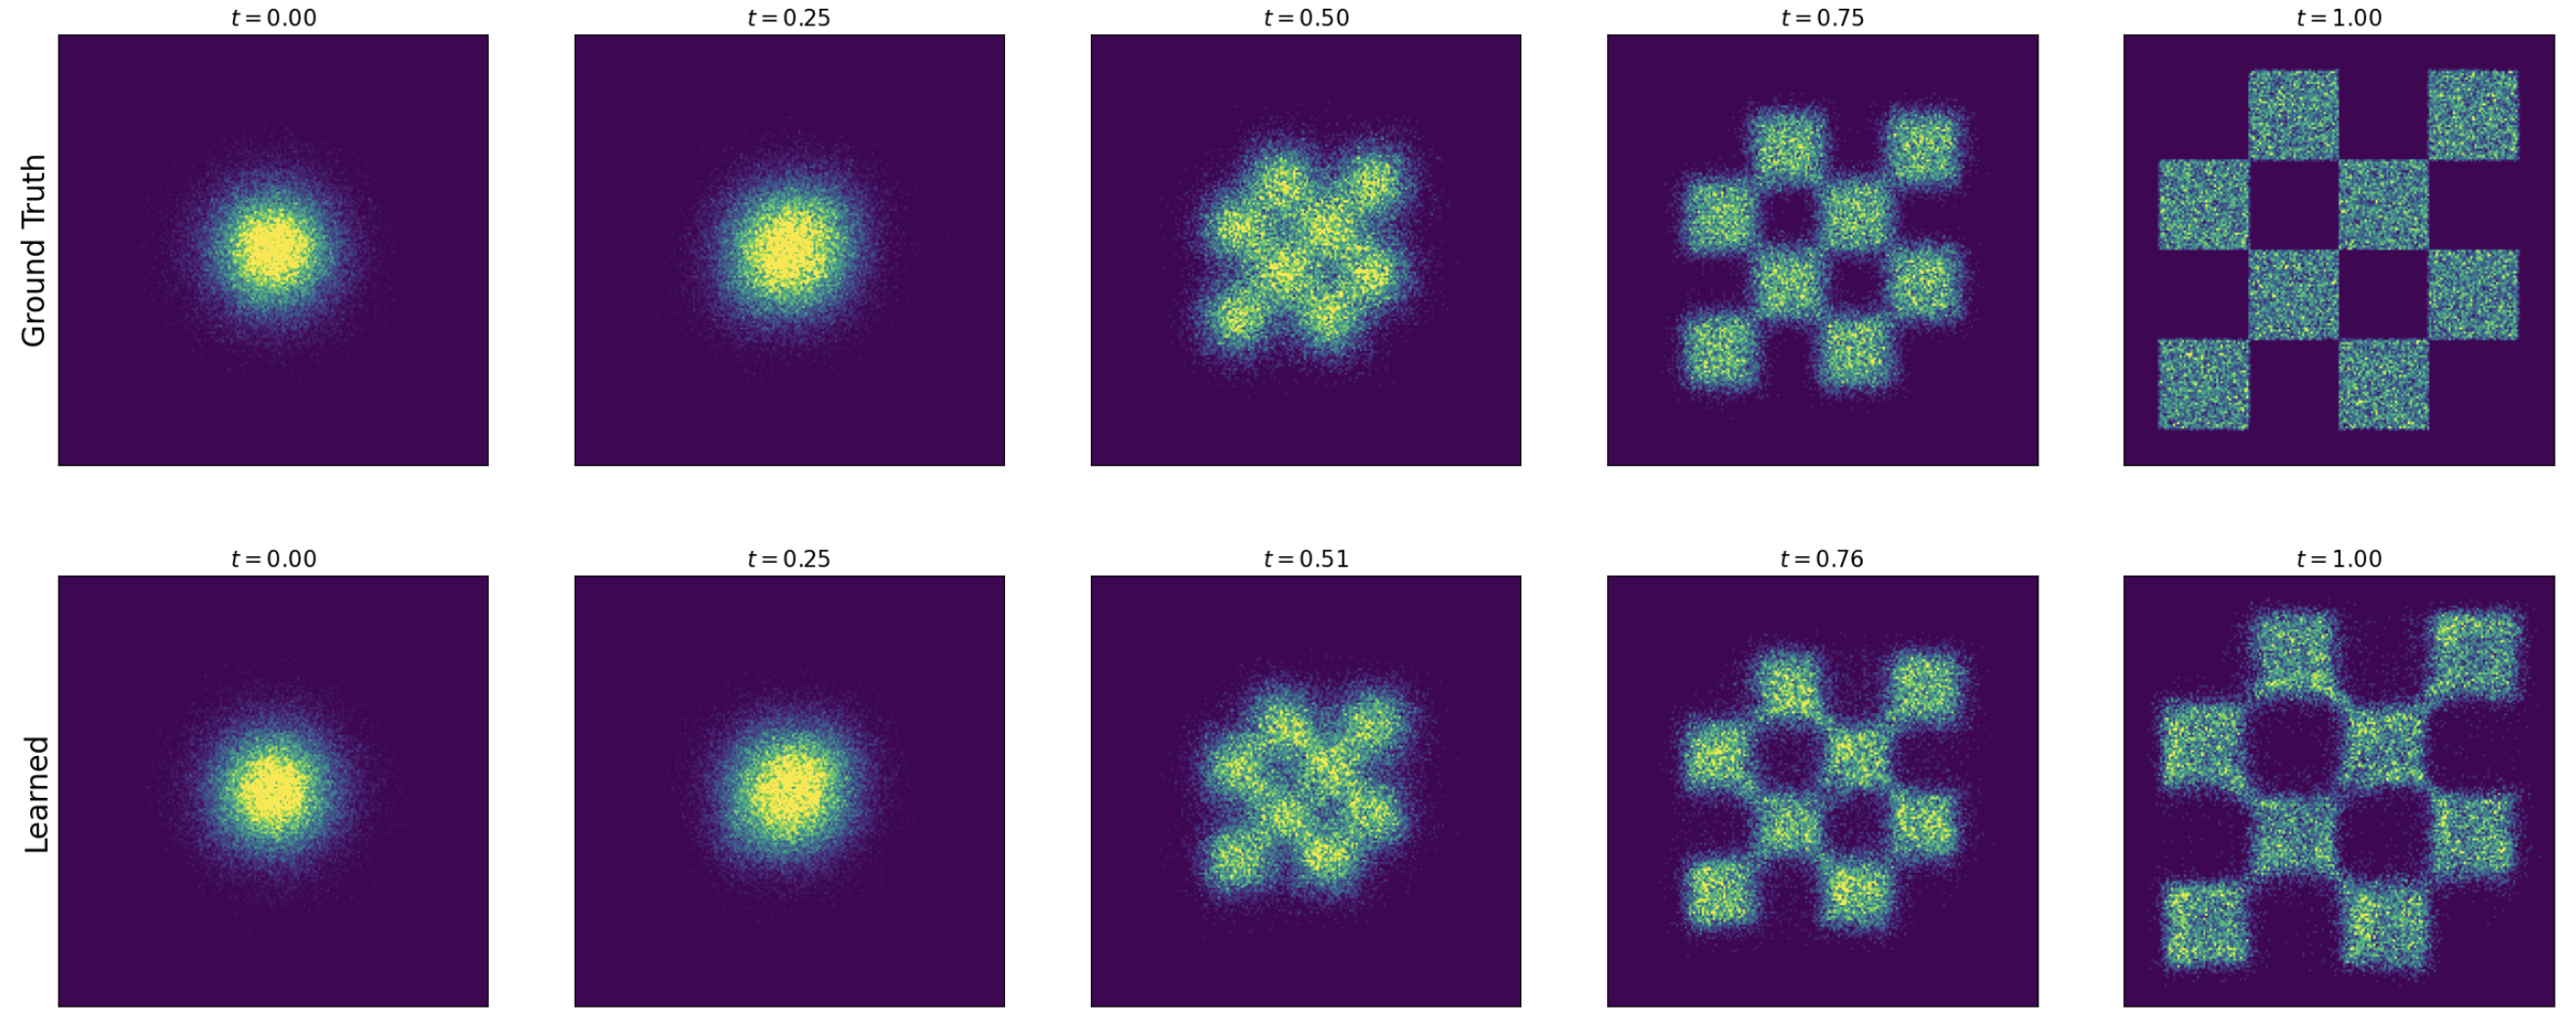
\includegraphics[width=0.95\linewidth]{tex/figures/selected/figure07-flow-matching.png}
  \caption{Flow Matching 训练后的 ODE 采样效果。上排是真实边缘概率路径，下排是训练后的 flow model 产生的样本分布。}
  \label{fig:flow-matching-simulation}
\end{figure}

如图~\ref{fig:flow-matching-simulation} 所示，训练充分时，flow matching 模型模拟出的分布会沿着预设概率路径逐步从噪声移动到数据。

\begin{algorithm}
\caption{Flow Matching Training Procedure for Gaussian CondOT Path}
\begin{algorithmic}[1]
\Require Dataset samples $z \sim \data$, neural network vector field $u_t^\theta$
\For{each mini-batch}
    \State Sample data $z$ from the dataset
    \State Sample time $t \sim \mathrm{Unif}[0,1]$
    \State Sample noise $\varepsilon \sim \Normal(0,I_d)$
    \State Set $x = t z + (1-t)\varepsilon$
    \State Compute loss
    \[
    \mathcal{L}(\theta)
    =
    \left\|
    u_t^\theta(x)-(z-\varepsilon)
    \right\|^2
    \]
    \State Update $\theta$ by a gradient step on $\mathcal{L}(\theta)$
\EndFor
\end{algorithmic}
\end{algorithm}

训练完成后，采样阶段只需要回到普通 flow model：
\begin{equation}
X_0 \sim p_{\mathrm{init}},
\qquad
\frac{\dd X_t}{\dd t}=u_t^\theta(X_t),
\end{equation}
并从 $t=0$ 模拟到 $t=1$。
如果训练充分好，则 $u_t^\theta$ 近似边缘目标向量场，最终样本 $X_1$ 就近似服从数据分布 $\data$。

\begin{summarybox}
Flow Matching 训练的核心在于学习边缘向量场 $u_t^{\mathrm{target}}$。为了构建它，我们选择一条满足 $p_0(\cdot|z) = p_{\mathrm{init}}$ 且 $p_1(\cdot|z) = \delta_z$ 的条件概率路径 $p_t(x|z)$。接下来，我们寻找一个条件向量场 $u_t^{\mathrm{target}}(x|z)$，使其对应的流 $\psi_t^{\mathrm{target}}(x|z)$ 满足：

\begin{equation}
X_0 \sim p_{\mathrm{init}} \Rightarrow X_t = \psi_t^{\mathrm{target}}(X_0|z) \sim p_t(\cdot|z)
\end{equation}

或者等价地，使 $u_t^{\mathrm{target}}$ 满足连续性方程。那么，由下式定义的边缘向量场：

\begin{equation}
u_t^{\mathrm{target}}(x) = \int u_t^{\mathrm{target}}(x|z) \frac{p_t(x|z)\data(z)}{p_t(x)} dz
\end{equation}

将遵循边缘概率路径，即：

\begin{equation}
X_0 \sim p_{\mathrm{init}}, dX_t = u_t^{\mathrm{target}}(X_t)dt \Rightarrow X_t \sim p_t \quad (0 \leq t \leq 1)
\end{equation}

特别地，对于该常微分方程（ODE），$X_1 \sim \data$，从而实现 $u_t^{\mathrm{target}}$ 将“噪声转化为数据”的预期目标。为了学习该向量场，我们最小化条件流匹配损失：

\begin{equation}
\mathcal{L}_{\text{CFM}}(\theta) = \mathbb{E}_{t \sim \text{Unif}, z \sim \data, x \sim p_t(\cdot|z)}[\|u_t^\theta(x) - u_t^{\mathrm{target}}(x|z)\|^2]
\end{equation}

最广泛使用的示例是高斯概率路径。在这种情况下，公式变为：

\begin{equation}
p_t(x|z) = \mathcal{N}(x; \alpha_t z, \beta_t^2 I_d)
\end{equation}

\begin{equation}
u_t^{\text{flow}}(x|z) = \left( \dot{\alpha}_t - \frac{\dot{\beta}_t \alpha_t}{\beta_t} \right) z + \frac{\dot{\beta}_t}{\beta_t} x
\end{equation}

\begin{equation}
\mathcal{L}_{\text{CFM}}(\theta) = \mathbb{E}_{t \sim \text{Unif}, z \sim \data, \varepsilon \sim \mathcal{N}(0, I_d)}[\|u_t^\theta(\alpha_t z + \beta_t \varepsilon) - (\dot{\alpha}_t z + \dot{\beta}_t \varepsilon)\|^2]
\end{equation}

其中噪声调度器 $\alpha_t, \beta_t \in \mathbb{R}$ 是连续可微且单调的函数，我们选择它们满足 $\alpha_0 = \beta_1 = 0$ 且 $\alpha_1 = \beta_0 = 1$（例如，$\alpha_t = t, \beta_t = 1 - t$）。
\end{summarybox}
